\documentclass[paper=a4,fontsize=12pt,ngerman]{scrartcl}

\usepackage[utf8]{inputenc} 
\usepackage[T1]{fontenc}
\usepackage{graphicx}
\usepackage[ngerman]{babel}
\usepackage{amsmath}
\usepackage[a4paper,left=25mm,right=25mm,top=25mm,bottom=30mm]{geometry}
\usepackage{parskip}
\usepackage{url}
\usepackage{multirow}
\usepackage{tabularx}
\usepackage{hyperref,amssymb}
\usepackage{paralist}
\usepackage{xcolor}

\usepackage{enumitem}

\definecolor{rosa}{HTML}{DF0174}

\newlist{titemize}{itemize}{1}% neue Listenumgebung für Tabellen
\setlist[titemize]{leftmargin=*,nosep,label=-}
% 


\begin{document}
	\pagenumbering{roman}
	\pagestyle{plain}
	
	% Einbinden der Titelseite
	
	\begin{titlepage}
	
	\linespread{1.5}
	
	
\includegraphics[width=\linewidth]{graphics/htw_logo}
	
	\begin{center}
		\large
		\hfill
		\vfill
		\Large{\bfseries{\textcolor{rosa}{Houdini Introduction\\ - \\ Prozedurale Modellierung}}}
		\\
		\large
		von \\
		Jana Koch, Laura Wagner, \\ 
		Nedim Thull, Ali Said, Samantha Maaß
		
	\end{center}
	
	\vfill
	
	
	\vfill
	
	%% {\bfseries{\textcolor{rosa}{}}}\\
	
	
	
	\vfill
\end{titlepage}

	\pagenumbering{arabic}
	\section*{\textcolor{rosa}{Getting started:}}
	\begin{itemize}
		\item Download der Free Test Version von Houdini 18.5.532 from https://sidefx.com/download/
		\item Registrierung mit Username und E-Mail notwendig
		\item Anmeldung auf der Webseite bevor Download möglich ist
		\item Bei der Installation ist es ratsam, neben den bereits markierten Komponenten, direkt die 'SideFX Labs' zu installieren. Dies ist kein muss, spart allerdings Zeit falls man sie später doch benötigt. SideFX Labs ist ein Toolset zur Unterstützung von Aufgaben bei der Erstellung digitaler Inhalte. 
		\item Beim erstmaligen starten von Houdini muss eine Lizenz installiert werden, in unserem Fall die 'free Houdini Apprentice license'
	\end{itemize}

	\section*{\textcolor{rosa}{Interface:}}
	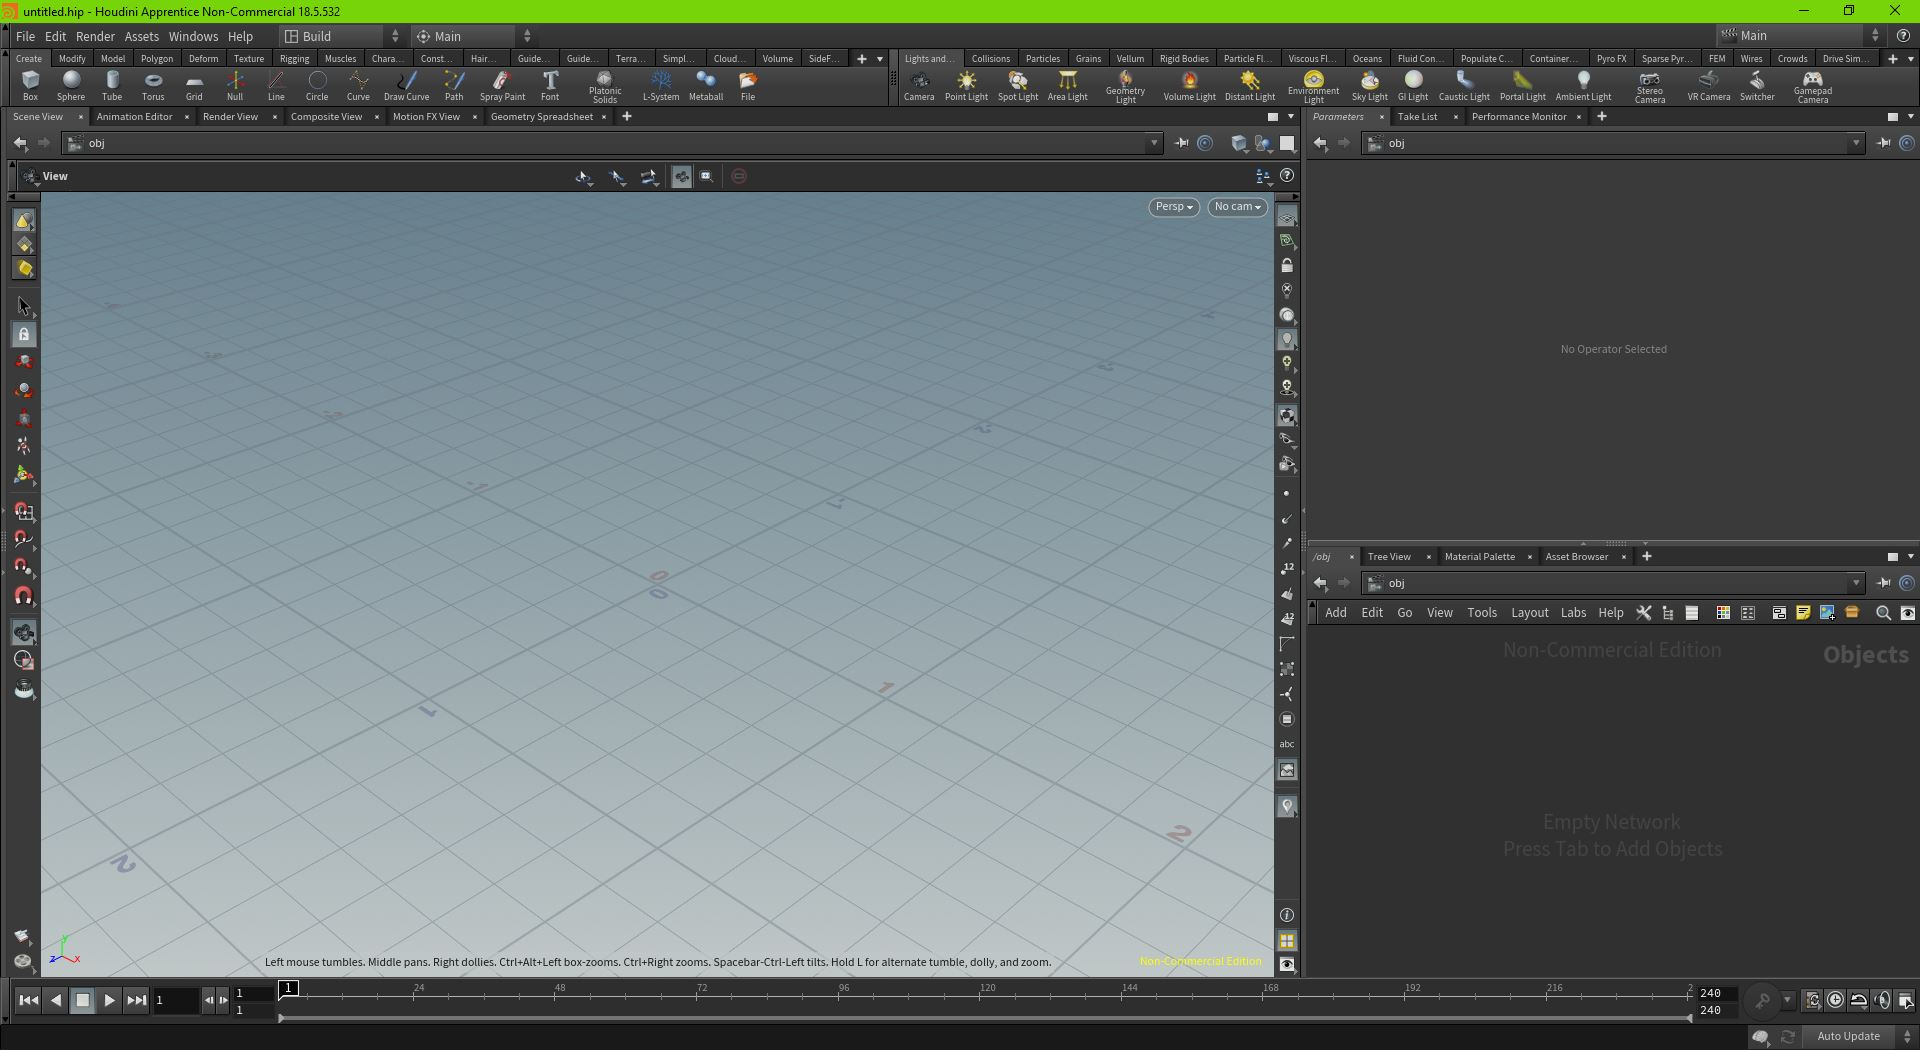
\includegraphics[width=\textwidth]{graphics/Interface.jpg}
	Das Standard-Interface ist in drei Teilbereiche aufgeteilt: 
	\begin{itemize}
		\item Die Scene View, eine 3D Ansicht der aktuellen Szene (links)
		\item Der Parameter Editor, zum anpassen der Parameter der aktuell ausgewählten Node. (rechts oben)
		\item Der Network Editor, zeigt alle Nodes des aktuellen Networks, man kann neue anlegen,sie miteinander verbinden und sie auswählen um die Parameter im Parameter Editor anzupassen. (rechts unten)
	\end{itemize}
		
		
\end{document}